% Lines starting with a percent sign (%) are comments. LaTeX will 
% not process those lines. Similarly, everything after a percent 
% sign in a line is considered a comment. To produce a percent sign
% in the output, write \% (backslash followed by the percent sign). 
% ==================================================================
% Usage instructions:
% ------------------------------------------------------------------
% The file is heavily commented so that you know what the various
% commands do. Feel free to remove any comments you don't need from
% your own copy. When redistributing the example thesis file, please
% retain all the comments for the benefit of other thesis writers! 
% ==================================================================
% Compilation instructions: 
% ------------------------------------------------------------------
% Use pdflatex to compile! Input images are expected as PDF files.
% Example compilation:
% ------------------------------------------------------------------
% > pdflatex thesis-example.tex
% > bibtex thesis-example
% > pdflatex thesis-example.tex
% > pdflatex thesis-example.tex
% ------------------------------------------------------------------
% You need to run pdflatex multiple times so that all the cross-references
% are fixed. pdflatex will tell you if you need to re-run it (a warning
% will be issued)  
% ------------------------------------------------------------------
% Compilation has been tested to work in ukk.cs.hut.fi and kosh.hut.fi
% - if you have problems of missing .sty -files, then the local LaTeX
% environment does not have all the required packages installed.
% For example, when compiling in vipunen.hut.fi, you get an error that
% tikz.sty is missing - in this case you must either compile somewhere
% else, or you cannot use TikZ graphics in your thesis and must therefore
% remove or comment out the tikz package and all the tikz definitions. 
% ------------------------------------------------------------------

% General information
% ==================================================================
% Package documentation:
% 
% The comments often refer to package documentation. (Almost) all LaTeX
% packages have documentation accompanying them, so you can read the
% package documentation for further information. When a package 'xxx' is
% installed to your local LaTeX environment (the document compiles
% when you have \usepackage{xxx} and LaTeX does not complain), you can 
% find the documentation somewhere in the local LaTeX texmf directory
% hierarchy. In ukk.cs.hut.fi, this is /usr/texlive/2008/texmf-dist,
% and the documentation for the titlesec package (for example) can be 
% found at /usr/texlive/2008/texmf-dist/doc/latex/titlesec/titlesec.pdf.
% Most often the documentation is located as a PDF file in 
% /usr/texlive/2008/texmf-dist/doc/latex/xxx, where xxx is the package name; 
% however, documentation for TikZ is in
% /usr/texlive/2008/texmf-dist/doc/latex/generic/pgf/pgfmanual.pdf
% (this is because TikZ is a front-end for PGF, which is meant to be a 
% generic portable graphics format for LaTeX).
% You can try to look for the package manual using the ``find'' shell
% command in Linux machines; the find databases are up-to-date at least
% in ukk.cs.hut.fi. Just type ``find xxx'', where xxx is the package
% name, and you should find a documentation file.
% Note that in some packages, the documentation is in the DVI file
% format. In this case, you can copy the DVI file to your home directory,
% and convert it to PDF with the dvipdfm command (or you can read the
% DVI file directly with a DVI viewer).
% 
% If you can't find the documentation for a package, just try Googling
% for ``latex packagename''; most often you can get a direct link to the
% package manual in PDF format.
% ------------------------------------------------------------------


% Document class for the thesis is report
% ------------------------------------------------------------------
% You can change this but do so at your own risk - it may break other things.
% Note that the option pdftext is used for pdflatex; there is no
% pdflatex option. 
% ------------------------------------------------------------------
\documentclass[12pt,a4paper,oneside,pdftex]{report}

% The input files (tex files) are encoded with the latin-1 encoding 
% (ISO-8859-1 works). Change the latin1-option if you use UTF8 
% (at some point LaTeX did not work with UTF8, but I'm not sure
% what the current situation is) 
\usepackage[utf8]{inputenc}
% OT1 font encoding seems to work better than T1. Check the rendered
% PDF file to see if the fonts are encoded properly as vectors (instead
% of rendered bitmaps). You can do this by zooming very close to any letter 
% - if the letter is shown pixelated, you should change this setting 
% (try commenting out the entire line, for example).  
\usepackage[OT1]{fontenc}
% The babel package provides hyphenating instructions for LaTeX. Give
% the languages you wish to use in your thesis as options to the babel
% package (as shown below). You can remove any language you are not
% going to use.
% Examples of valid language codes: english (or USenglish), british, 
% finnish, swedish; and so on.
\usepackage[finnish,swedish,english]{babel}


% Font selection
% ------------------------------------------------------------------
% The default LaTeX font is a very good font for rendering your 
% thesis. It is a very professional font, which will always be 
% accepted. 
% If you, however, wish to spicen up your thesis, you can try out
% these font variants by uncommenting one of the following lines
% (or by finding another font package). The fonts shown here are 
% all fonts that you could use in your thesis (not too silly). 
% Changing the font causes the layouts to shift a bit; you many
% need to manually adjust some layouts. Check the warning messages
% LaTeX gives you.
% ------------------------------------------------------------------
% To find another font, check out the font catalogue from
% http://www.tug.dk/FontCatalogue/mathfonts.html
% This link points to the list of fonts that support maths, but
% that's a fairly important point for master's theses.
% ------------------------------------------------------------------
% <rant>
% Remember, there is no excuse to use Comic Sans, ever, in any
% situation! (Well, maybe in speech bubbles in comics, but there 
% are better options for those too)
% </rant>

% \usepackage{palatino}
% \usepackage{tgpagella}



% Optional packages
% ------------------------------------------------------------------
% Select those packages that you need for your thesis. You may delete
% or comment the rest.

% Natbib allows you to select the format of the bibliography references.
% The first example uses numbered citations: 
% \usepackage[square,sort&compress,numbers]{natbib}
% The second example uses author-year citations.
% If you use author-year citations, change the bibliography style (below); 
% acm style does not work with author-year citations.
% Also, you should use \citet (cite in text) when you wish to refer
% to the author directly (\citet{blaablaa} said blaa blaa), and 
% \citep when you wish to refer similarly than with numbered citations
% (It has been said that blaa blaa~\citep{blaablaa}).
% \usepackage[square]{natbib}

\usepackage{csquotes}% Recommended
\usepackage[backend=biber, style=authoryear, urldate=comp, maxbibnames = 99]{biblatex}
\renewbibmacro{in:}{}
\DeclareFieldFormat{urldate}{\addcomma\space\bibstring{urlseen}\space#1}
\DefineBibliographyStrings{english}{%
  urlseen = {cited},
}
\addbibresource{sources.bib}% Syntax for version >= 1.2

% The alltt package provides an all-teletype environment that acts
% like verbatim but you can use LaTeX commands in it. Uncomment if 
% you want to use this environment. 
% \usepackage{alltt}

% The eurosym package provides a euro symbol. Use with \euro{}
\usepackage{eurosym} 

% Verbatim provides a standard teletype environment that renderes
% the text exactly as written in the tex file. Useful for code
% snippets (although you can also use the listings package to get
% automatic code formatting). 
\usepackage{verbatim}

% The listing package provides automatic code formatting utilities
% so that you can copy-paste code examples and have them rendered
% nicely. See the package documentation for details.
% \usepackage{listings}

% The fancuvrb package provides fancier verbatim environments 
% (you can, for example, put borders around the verbatim text area
% and so on). See package for details.
% \usepackage{fancyvrb}

% Supertabular provides a tabular environment that can span multiple 
% pages. 
%\usepackage{supertabular}
% Longtable provides a tabular environment that can span multiple 
% pages. This is used in the example acronyms file. 
\usepackage{longtable}

% The fancyhdr package allows you to set your the page headers 
% manually, and allows you to add separator lines and so on. 
% Check the package documentation. 
% \usepackage{fancyhdr}

% Subfigure package allows you to use subfigures (i.e. many subfigures
% within one figure environment). These can have different labels and
% they are numbered automatically. Check the package documentation. 
\usepackage{subfigure}

% The titlesec package can be used to alter the look of the titles 
% of sections, chapters, and so on. This example uses the ``medium'' 
% package option which sets the titles to a medium size, making them
% a bit smaller than what is the default. You can fine-tune the 
% title fonts and sizes by using the package options. See the package
% documentation.
\usepackage[medium]{titlesec}

% The TikZ package allows you to create professional technical figures.
% The learning curve is quite steep, but it is definitely worth it if 
% you wish to have really good-looking technical figures. 
\usepackage{tikz}
% You also need to specify which TikZ libraries you use
\usetikzlibrary{positioning}
\usetikzlibrary{calc}
\usetikzlibrary{arrows}
\usetikzlibrary{decorations.pathmorphing,decorations.markings}
\usetikzlibrary{shapes}
\usetikzlibrary{patterns}


% The aalto-thesis package provides typesetting instructions for the
% standard master's thesis parts (abstracts, front page, and so on)
% Load this package second-to-last, just before the hyperref package.
% Options that you can use: 
%   mydraft - renders the thesis in draft mode. 
%             Do not use for the final version. 
%   doublenumbering - [optional] number the first pages of the thesis
%                     with roman numerals (i, ii, iii, ...); and start
%                     arabic numbering (1, 2, 3, ...) only on the 
%                     first page of the first chapter
%   twoinstructors  - changes the title of instructors to plural form
%   twosupervisors  - changes the title of supervisors to plural form
%\usepackage[mydraft,twosupervisors]{aalto-thesis}
\usepackage[mydraft,doublenumbering]{aalto-thesis}
%\usepackage{aalto-thesis}



% Hyperref
% ------------------------------------------------------------------
% Hyperref creates links from URLs, for references, and creates a
% TOC in the PDF file.
% This package must be the last one you include, because it has
% compatibility issues with many other packages and it fixes
% those issues when it is loaded.   
%\RequirePackage[pdftex]{hyperref}
\RequirePackage[pdfa]{hyperref}
% Setup hyperref so that links are clickable but do not look 
% different
\hypersetup{colorlinks=false,raiselinks=false,breaklinks=true}
\hypersetup{pdfborder={0 0 0}}
\hypersetup{bookmarksnumbered=true}
% The following line suggests the PDF reader that it should show the 
% first level of bookmarks opened in the hierarchical bookmark view. 
\hypersetup{bookmarksopen=true,bookmarksopenlevel=1}
% Hyperref can also set up the PDF metadata fields. These are
% set a bit later on, after the thesis setup.   


% Thesis setup
% ==================================================================
% Change these to fit your own thesis.
% \COMMAND always refers to the English version;
% \FCOMMAND refers to the Finnish version; and
% \SCOMMAND refers to the Swedish version.
% You may comment/remove those language variants that you do not use
% (but then you must not include the abstracts for that language)
% ------------------------------------------------------------------
% If you do not find the command for a text that is shown in the cover page or
% in the abstract texts, check the aalto-thesis.sty file and locate the text
% from there. 
% All the texts are configured in language-specific blocks (lots of commands
% that look like this: \renewcommand{\ATCITY}{Espoo}.
% You can just fix the texts there. Just remember to check all the language
% variants you use (they are all there in the same place). 
% ------------------------------------------------------------------
\newcommand{\TITLE}{Selling services for private housing companies}
\newcommand{\FTITLE}{Palveluiden myynti taloyhtiöille}
%\newcommand{\STITLE}{Den stora stygga vargen:}
\newcommand{\SUBTITLE}{Bringing customers into focus}
\newcommand{\FSUBTITLE}{Asiakkaat keskiöön}
%\newcommand{\SSUBTITLE}{Lilla Vargens universum}
\newcommand{\DATE}{February 14, 2018}
\newcommand{\FDATE}{14. helmikuuta 2018}
%\newcommand{\SDATE}{Den 18 februari 2018}

% Supervisors and instructors
% ------------------------------------------------------------------
% Usually thesis have one supervisor and one advisor. Sometimes you
% may have two advisors and, in double degree
% programs, you may have two supervisors. 
% If you have two supervisors, write both names here, separate them with a 
% double-backslash (see below for an example)
% Also remember to add the package option ``twosupervisors'' or
% ``twoinstructors'' to the aalto-thesis package (aalto-thesis.sty
% file line 72), so that the titles are in plural.
% Example of one supervisor:
\newcommand{\SUPERVISOR}{Professor Risto Sarvas, Aalto University}
\newcommand{\FSUPERVISOR}{Professori Risto Sarvas, Aalto-yliopisto}
%\newcommand{\SSUPERVISOR}{Professor Antti Ylä-Jääski}
% Example of twosupervisors:
%\newcommand{\SUPERVISOR}{Professor Antti Ylä-Jääski\\ Professor Petra Perustieteilijä}
% \newcommand{\FSUPERVISOR}{Professori Antti Ylä-Jääski\\ Professori Petra Perustieteilijä}
%\newcommand{\SSUPERVISOR}{Professor Antti Ylä-Jääski\\ Professor Petra Perustieteilijä}

% If you have only one instructor, just write one name here
\newcommand{\INSTRUCTOR}{Minna Näsman, Dr.Theol.}
\newcommand{\FINSTRUCTOR}{Minna Näsman, TT}
%\newcommand{\SINSTRUCTOR}{Diplomingenjör Oili Ohjaaja}
% If you have two instructors, separate them with \\ to create linefeeds
% \newcommand{\INSTRUCTOR}{Oili Ohjaaja M.Sc. (Tech.)\\
%  Elli Opas M.Sc. (Tech)}
%\newcommand{\FINSTRUCTOR}{Diplomi-insinööri Oili Ohjaaja\\
%  Diplomi-insinööri Elli Opas}
%\newcommand{\SINSTRUCTOR}{Diplomingenjör Oili Ohjaaja\\
%  Diplomingenjör Elli Opas}

% If you have two supervisors, it is common to write the schools
% of the supervisors in the cover page. If the following command is defined,
% then the supervisor names shown here are printed in the cover page. Otherwise,
% the supervisor names defined above are used.
%\newcommand{\COVERSUPERVISOR}{Professor Risto Sarvas Aalto University}

% The same option is for the instructors, if you have multiple instructors.
% \newcommand{\COVERINSTRUCTOR}{Oili Ohjaaja M.Sc. (Tech.), Aalto University\\
%  Elli Opas M.Sc. (Tech), Aalto SCI}


% Other stuff
% ------------------------------------------------------------------
\newcommand{\PROFESSORSHIP}{Information Networks}
\newcommand{\FPROFESSORSHIP}{Informaatioverkostot}
%\newcommand{\SPROFESSORSHIP}{Datateknik}
% Professorship code is the same in all languages
\newcommand{\PROFCODE}{SCI3042}
\newcommand{\KEYWORDS}{ocean, sea, marine, ocean mammal, marine
  mammal, whales, cetaceans, dolphins}
\newcommand{\FKEYWORDS}{aineistot, aitta, akustiikka, Alankomaat,
aluerakentaminen, aapinen, ankka, aasinsilta}
%\newcommand{\SKEYWORDS}{omsättning, kassaflöde, värdepappersmarknadslagen,
%yrkesutövare, intresseföretag, verifieringskedja}
\newcommand{\LANGUAGE}{English}
\newcommand{\FLANGUAGE}{Englanti}
%\newcommand{\SLANGUAGE}{Engelska}

% Author is the same for all languages
\newcommand{\AUTHOR}{Anna Hurtta}


% Currently the English versions are used for the PDF file metadata
% Set the PDF title
\hypersetup{pdftitle={\TITLE\ \SUBTITLE}}
% Set the PDF author
\hypersetup{pdfauthor={\AUTHOR}}
% Set the PDF keywords
\hypersetup{pdfkeywords={\KEYWORDS}}
% Set the PDF subject
\hypersetup{pdfsubject={Master's Thesis}}


% Layout settings
% ------------------------------------------------------------------

% When you write in English, you should use the standard LaTeX 
% paragraph formatting: paragraphs are indented, and there is no 
% space between paragraphs.
% When writing in Finnish, we often use no indentation in the
% beginning of the paragraph, and there is some space between the 
% paragraphs. 

% If you write your thesis Finnish, uncomment these lines; if 
% you write in English, leave these lines commented! 
% \setlength{\parindent}{0pt}
% \setlength{\parskip}{1ex}

% Use this to control how much space there is between each line of text.
% 1 is normal (no extra space), 1.3 is about one-half more space, and
% 1.6 is about double line spacing.  
% \linespread{1} % This is the default
% \linespread{1.3}

% Bibliography style
% acm style gives you a basic reference style. It works only with numbered
% references.
% bibliographystyle{acm}
% Plainnat is a plain style that works with both numbered and name citations.
% \bibliographystyle{plainnat}


% Extra hyphenation settings
% ------------------------------------------------------------------
% You can list here all the files that are not hyphenated correctly.
% You can provide many \hyphenation commands and/or separate each word
% with a space inside a single command. Put hyphens in the places where
% a word can be hyphenated.
% Note that (by default) LaTeX will not hyphenate words that already
% have a hyphen in them (for example, if you write ``structure-modification 
% operation'', the word structure-modification will never be hyphenated).
% You need a special package to hyphenate those words.
\hyphenation{di-gi-taa-li-sta yksi-suun-tai-sta}



% The preamble ends here, and the document begins. 
% Place all formatting commands and such before this line.
% ------------------------------------------------------------------
\begin{document}
% This command adds a PDF bookmark to the cover page. You may leave
% it out if you don't like it...
\pdfbookmark[0]{Cover page}{bookmark.0.cover}
% This command is defined in aalto-thesis.sty. It controls the page 
% numbering based on whether the doublenumbering option is specified
\startcoverpage

% Cover page
% ------------------------------------------------------------------
% Options: finnish, english, and swedish
% These control in which language the cover-page information is shown
\coverpage{english}


% Abstracts
% ------------------------------------------------------------------
% Include an abstract in the language that the thesis is written in,
% and if your native language is Finnish or Swedish, one in that language.

% Abstract in English
% ------------------------------------------------------------------
\thesisabstract{english}{
The abstract provides goal, motivation, background, and conclusions of
the work. It has to fit to one page together with the bibliographical
information. 

If the thesis is in English and the language of school
education is Finnish or Swedish, the abstract is written in English
and in Finnish or in Swedish. If the language of school education is
other than Finnish or Swedish, the abstract is written in English only.

The thesis example file (\texttt{thesis-example.tex}), all the chapter content
files (\texttt{1introduction.tex} and so on), and the Aalto style file
(\texttt{aalto-thesis.sty}) are commented with explanations on how the Aalto
thesis works. The files also contain some examples on how to customize various
details of the thesis layout, and of course the example text works as an
example in itself. Please read the comments and the example text; that should
get you well on your way!

In the thesis template, you can find the text of the abstract in the
abstract in the \texttt{thesis-example.tex}
file, together with the bibliographical information of the abstract tables.
\fixme{This is an example how to use fixme: add your abstract here.} 
Fixme is a command that helps you identify parts of your thesis that still
require some work. When compiled in the custom \texttt{mydraft} mode, text
parts tagged with fixmes are shown in bold and with fixme tags around them. When
compiled in normal mode, the fixme-tagged text is shown normally (without
special formatting). The draft mode also causes the ``Draft'' text to appear on
the front page, alongside with the document compilation date. The custom
\texttt{mydraft} mode is selected by the \texttt{mydraft} option given for the
package \texttt{aalto-thesis}, near the top of the \texttt{thesis-example.tex}
file.

The instructions on how to compile LaTeX *.tex files to *.pdf files like this 
are giving in the \texttt{thesis-example.tex} file as comments and also in this 
pdf in a Section~\ref{section:compilation}.}

% Abstract in Finnish
% ------------------------------------------------------------------
\thesisabstract{finnish}{
Jos koulusivistyskielesi on suomi, diplomityössä pitää olla
suomenkielinen tiivistelmä. Tiivistelmän pitää mahtua yhdelle
sivulle.

Tiivistelmässä on yleensä useampia kappaleita. Tiivistelmä kertoo työn
tavoitteet, motivaation, taustan ja johtopäätökset.
}

% Acknowledgements
% ------------------------------------------------------------------
% Select the language you use in your acknowledgements
\selectlanguage{english}

% Uncomment this line if you wish acknoledgements to appear in the 
% table of contents
%\addcontentsline{toc}{chapter}{Acknowledgements}

% The star means that the chapter isn't numbered and does not 
% show up in the TOC
\chapter*{Acknowledgements}

It has been a long and bumpy road to this point where I can say that I am done with school.

Thank you, and keep up the good work!
\vskip 10mm

\noindent Espoo, \DATE
\vskip 5mm
\noindent\AUTHOR

% Acronyms
% ------------------------------------------------------------------
% Use \cleardoublepage so that IF two-sided printing is used 
% (which is not often for masters theses), then the pages will still
% start correctly on the right-hand side.
\cleardoublepage
% Example acronyms are placed in a separate file, acronyms.tex
\addcontentsline{toc}{chapter}{Abbreviations and Acronyms}
\chapter*{Abbreviations and Acronyms}

% The longtable environment should break the table properly to multiple pages, 
% if needed

\noindent
\begin{longtable}{@{}p{0.25\textwidth}p{0.7\textwidth}@{}}
2k/4k/8k mode & COFDM operation modes \\
3GPP & 3rd Generation Partnership Project \\ 
ESP & Encapsulating Security Payload; An IPsec security protocol \\ 
FLUTE  & The File Delivery over Unidirectional Transport protocol \\ 
e.g.& for example (do not list here this kind of common acronymbs or abbreviations, but only those that are essential for understanding the content of your thesis. \\ 
note & Note also, that this list is not compulsory, and should be omitted if you have only few abbreviations

\end{longtable}


% Table of contents
% ------------------------------------------------------------------
\cleardoublepage
% This command adds a PDF bookmark that links to the contents.
% You can use \addcontentsline{} as well, but that also adds contents
% entry to the table of contents, which is kind of redundant.
% The text ``Contents'' is shown in the PDF bookmark. 
\pdfbookmark[0]{Contents}{bookmark.0.contents}
\tableofcontents

% List of tables
% ------------------------------------------------------------------
% You only need a list of tables for your thesis if you have very 
% many tables. If you do, uncomment the following two lines.
% \cleardoublepage
% \listoftables

% Table of figures
% ------------------------------------------------------------------
% You only need a list of figures for your thesis if you have very 
% many figures. If you do, uncomment the following two lines.
% \cleardoublepage
% \listoffigures

% The following label is used for counting the prelude pages
\label{pages-prelude}
\cleardoublepage

%%%%%%%%%%%%%%%%% The main content starts here %%%%%%%%%%%%%%%%%%%%%
% ------------------------------------------------------------------
% This command is defined in aalto-thesis.sty. It controls the page 
% numbering based on whether the doublenumbering option is specified
\startfirstchapter

% Add headings to pages (the chapter title is shown)
\pagestyle{headings}

% The contents of the thesis are separated to their own files.
% Edit the content in these files, rename them as necessary.
% ------------------------------------------------------------------
\chapter{Introduction}
\label{chapter:intro}

This master's thesis purpose is to find out how to sell services for limited liability housing companies in a situation where the case company sells the service for another company and then to the end customer. The study uses design science research approach and it is conducted as a service design project.

This chapter begins by presenting the background and motivation for the research and introducing the case company. Then the problem and research questions are described and finally, the structure of the thesis is presented.

\section{Background and motivation}

In Finland about 2,7 million people are living in approximately 88 000 limited liability housing companies \parencite{REMF, Stats}. This limited liability housing company regime is an unique setting compared to other countries and it is dominant form of ownership in multi-apartment buildings in Finland \parencite{Lujanen:2017}. The operation of the limited liability company is regulated in the Finnish law \parencite{YIT}.

There are a lot of books and online material to support and guidance the people who are in the board of a limited liability housing company. In addition, it is discussed a lot that the work in a limited liability housing company can be a hassle and people do not want to participate in the operation of the housing company. However, there is a lack of knowledge and understanding about the buying decision making process as well as the motivation of the people to be in the board.

This study tries to fill the knowledge gap by researching and understanding the people who are working in a limited liability housing company and create a better way to reach the thousands of limited liability housing companies by identifying some similarities between them.

Related to the energy industry this study concentrates, the aim is to facilitate a more customer-centric approach since according to \textcite{Fader:2012} enegy firms do not refer to their customers as \emph{customers} but \emph{rate-payers}. This emphasizes how the energy firms view their customers as homogenous and what could be changed.

\section{Introduction to case company}

The case company in this study is Leanheat which provides a software solution that enables the space  heating optimization of centrally heated multi-family residential buildings. This is done by installing wireless sensors to track temperature and humidity, and a connection to the central heating controller is established. The system collects data from apartments, heating system and weather in order to automatically create a thermodynamic model for the building. Then the space heating is optimized based on the parameters resulting a minimized simultaneous usage of heat and thus lowering the peak loads caused by it. \parencite{LenheatArticle:2019}

The traditional heating system can not adjust to the changing weather or the thermodynamic properties of the building. In addition, the traditional system does not communicate with other systems inside the buildings nor with the buildings within the same network. This causes a suboptimal behaviour in the system, since it possible that all of these components require high heat power at the same time. \parencite{LenheatArticle:2019}

The benefits of the Leanheat's solution for district heating companies are that 1) the peak loads are 20 \% lower and primary return temperatures are two to four degrees lower, 2) heat production is optimized with demand forecasts and demand response and 3) data from the buildings offer new business models to be used and developed. For residents the solution provides stable and better indoor conditions. \parencite{LenheatArticle:2019}

In Finland, from the big apartment buildings around one third is owned by the professional property owners and in that specific market the case company is already the market lead. The rest of the buildings are limited liability housing companies which means that reaching them as clients is strategically important in order to grow bigger in the market.

Leanheat and district heating companies are forming partnerships because the system provides a way for the district heating companies to optimize their energy production. Moreover, based on the research done by \textcite{Energyindustry:2019} customers are becoming active in acquiring services which means that the energy companies should be more active in providing service business in order to engage better with their customers.

\section{Problem statement}

As stated above, acquiring limited liability housing companies as clients is difficult, because there are tens of thousands of them and those are run by laypersons. In addition, most of them operate in "status quo" which means that the goal of the private housing company is to keep the building as it is rather than developing it. Selling services for limited liability housing companies requires resources and knowledge about the end customer. On top of that, district heating companies are valuable since currently they have their exiting customer relationships with limited liability housing companies because they provide them heat.

The research will concentrate on creating new and better understanding on the buying decision making processes inside limited liability housing companies by exploring the background motivation for people to be in the board and what affects the decision making. With that understanding it is then possible to design and develop a sales process and guidelines on how to reach the potential market of the limited liability housing companies. Thus, the first research question is formed as follows:\\\\
\emph{RQ1: What affects the purchasing decision making process in a limited liability housing companies?}\\

In addition, the partnerships should be taken into account when designing and developing in order to find out the value for district heating companies. By doing this research the aim is to create a new service business opportunity and by concrete increase sales, reduce lead times and customer acquisition costs. To answer this, the second research question is formulated as follows:\\\\
\emph{RQ2: What kind of sales process could help engage the end-customer in B2B2C setting?}\\

\section{Structure of the Thesis}
\label{section:structure} 

In the next chapter, the background information about limited liability housing companies is studied and presented to gain understanding about what they are and how they operate. In addition, Chapter ~\ref{chapter:background} present the environment concerning the energy business and its key features related to service business and future development. The research methods are presented in Chapter ~\ref{chapter:methods} along with the description on how the methods were implemented in the study. In Chapter ~\ref{chapter:results} the results of the study are presented. Finally, the discussion related to the results of the study as well as limitations of the study and future research are discussed in the Chapter ~\ref{chapter:discussion}.

\chapter{Background}
\label{chapter:background} 

This section introduces the theoretical background of the thesis. First the l

\section{Limited Liability Housing Company}

In this chapter the regime of limited liability housing company is presented and the operation of it is described in order to provide background information. First the basic concept is explained, then the responsibilities and operation of the limited liability housing company is presented.

Limited liability housing company is a type of limited liability company whose purpose is to own and control one or multiple building or a part of it where over the half of the combined floor surface area of the apartment or apartments is designated in the articles of association to be possessed by the shareholders and to be used as residential apartments \parencite{LLHA:2}. To put it simple, the company owns the property and the share capital is divided into shares. For the shareholders, these shares then give a right of possession to a specific apartment. \parencite{Lujanen:2017}. So, when a person buys an apartment in a limited liability housing company, she become the shareholder of the bought apartment \parencite{YIT}.

In Finland about 2,7 million people are living in approximately 88 000 limited liability housing companies \parencite{REMF, Stats}. This limited liability housing company regime is an unique setting compared to other countries and it is dominant form of ownership in multi-apartment buildings in Finland \parencite{Lujanen:2017}. The operation of the limited liability company is regulated in the Finnish law and the articles of association contains the internal law and order of the specific housing company \parencite{YIT}. In practice, the limited liability housing company takes care of the real estates and buildings to which it controls \parencite{LLHA:2}. 

\subsection{The Division of Responsibilities}

Limited liability housing company is led by the board and deputy landlord and their job is to act in a way that advances the company's interest \parencite{LLHA:2}. However, this does not mean that the people who are in the board should have expertise in the real estate field. So, the people working in the board are mostly laypersons which should be considered inside the board as well as among the shareholders. \parencite{Hallintotapa:2017}

The highest decision-making body is the shareholder's meeting which is held once a year. In a shareholder's meeting every shareholder has a right to vote. Shareholders one of the most important responsibility is to decide who will be in the board of the limited liability housing company. The Table~\ref{table:responsibilities} presents the actors who form the limited liability housing company and their responsibilities in addition to the previously mentioned. \parencite{RantanenViiala:2015} 

\begin{table}
\begin{tabular}{|p{2.5cm}|p{2.5cm}|p{6.4cm}|} 
\hline % The line on top of the table
\textbf{Organ} & \textbf{Chooser}  & \textbf{Responsibilities} \\ 
\hline 
Shareholder's meeting & Formed by all shareholders, not chosen & Shareholder's meeting decide on financial statement, maintenance fee, loans and major overhauls. Shareholder's meeting chooses the board members and gives the freedom of responsibility for the board members and the deputy landlord. In addition they chooses the auditor.\\ 
\hline
Board & Shareholder's meeting & The board chooses the deputy landlord, if the board do not take care of the real estate management by themselves. Board accepts the agreements and oversees the finance. Additionally the board makes a five year plan which covers the needed renovations and repairs. The board also presents the renovations done previously.\\
\hline
Deputy landlord & Board & Deputy landlord's responsibility is to take care of the daily operations of the limited liability housing company. Deputy landlord executes the decisions which the board has made. In addition deputy landlord prepares the board meetings and act as a secretary.\\
\hline
Service company & Board & Service company operates under deputy landlord and they do all tasks agreed on the agreements, for example cleaning of the public spaces.\\
\hline
Auditor & Shareholder's meeting & Auditor checks the company's accounts and the legality of the government. Auditor is responsible to report the status for the shareholder's meeting.\\
\hline
\end{tabular} % for really simple tables, you can just use tabular
% You can place the caption either below (like here) or above the table
\caption{Limited liability housing company's organs and their responsibilities. \parencite{RantanenViiala:2015}}
% Place the label just after the caption to make the link work
\label{table:responsibilities}
\end{table} % table makes a floating object with a title

The shareholder's meeting is a place where the shareholders, board members and the deputy landlord meet each other and the meeting provides a good place for discussions and questions \parencite{Hallintotapa:2017}. The decision making in a shareholder's meeting happens usually with the majority decision, which means that the suggestion which has over half of the votes is the final decision. If the voting is related to person, the one who receives most of the votes gets elected. In tie situation the chairperson makes the decision, if the voting is not related to electing a person. \parencite{RantanenViiala:2015}

In the shareholder's meeting the housing board's responsibility is to present the scope of the maintenance actions to be done in the limited liability housing company. This scope is then decided in the meeting. \parencite{RantanenViiala:2015} Based on the \textcite{LLHA:2} the board requires shareholder's meeting's decision to proceed with actions which are considering the size and operation of the company unusual or far-reaching, affecting essentially to the use of the shareholder's apartment or affecting essentially to the obligation to pay maintenance fee or to other expenses which are caused by the use of the shareholder's possessed apartment.

The role of the deputy landlord is similar to the managing director in a limited liability company since it is the deputy landlord's responsibility to take care of the daily administration.  Additionally, deputy landlord puts in action the decisions made by the housing board and takes care that the accounting is done properly according to the law. \parencite{Sarekoski:2015}

\section{Energy Industry in Finland}

This chapter focuses on the energy industry and the ecosystem of it in Finland, but gives also an overview of the international energy transition.

In Finland there are around 100 district heating companies which are responsible for heat distribution, sale and production. Most of these companies are owned by the municipalities. \parencite{Energyindustry:2019,Poyry:2018} Based on the statistics made by \textcite{Energyindustrygraphs:2018} 46 \% of apartment buildings are part of the district heating network which means that 2,92 million residents are living in apartments which are heated with district heating.

\subsection{Energy Transition}

\emph{International Renewable Energy Agency IRENA} published report which discusses the energy transformation and actions needed to do in order to keep the global temperature rise below 2 degree Celsius by the year 2050. This transformation or to speak \emph{energy transition} in practice means going from energy  system that is based on fossil fuels to one which is more efficient and based on renewable energy.

The report states many problems which are not in track with the targets. However, in this thesis the researcher highlights only some of them which are more relevant regarding the thesis focus and scope. Such topic is energy efficiency. One of the facts stated in the report is that the main factors making energy transition to happen are energy efficiency and renewable energy. Together they could deliver 90\% of the required cut in energy-related CO2 emissions in the speed which is needed.

According to IRENA especially in the building sector the energy efficiency becomes more crucial factor in energy transition.  


\section{Customer Centricity}

\textcite{Drucker:2007} states in his book The Practice of Management that the purpose of a business is to create customers by business actions. Moreover the customers are the ones who determines what a business is. For the business, it is most important to understand what the customers consider as value since it is them who decides what the business produces. In addition, according to \textcite{Parniangtong:2017} organizations' performance have also been explained with the focus on the outcomes which the customers value and are willing to pay. This means, that the customers are more satisfied and thus give a competitive advantage for the company. For a company to succeed in nowadays competition in the marketplace, customer centricity is a must \parencite{PathToCustomerCentricity:2006}.

Customer-centric thinking is built on four main arguments which are as follows:
\begin{enumerate}
\item Loyal customers should produce more money for a company.
\item New customers might not produce money immediately, but they should be profitable for the company in the future.
\item  It is more affordable to serve and introduce new offerings to long-term customers than to new customers.
\item  Long-term customers are more stable when it comes to pricing and a company's digressions, in addition they are more likely to spread word about the company. \parencite{Parniangtong:2017}
\end{enumerate}

Based on these arguments, the loyal customers bring more value to the company and through this, the competitive advantage of the company becomes better. Because customer-centric thinking drives from the goal where the customer equity is on high level, the company should focus on the customer relationship over lifetime. In order to achieve customer equity the company should know their customers, respond to their needs, appreciate them and maintain a profitable relationship with them over a long time. \parencite{Parniangtong:2017}

\textcite{Parniangtong:2017} states that customer value is created by a value chain which is customer driven, being closer with the customer, selling solution, having trust from the customers and offering intimacy with their customers through personalized experience. Having a customer-driven value chain compared to the traditional product oriented, the company can serve customers' needs better because then the customer needs will drive the changed. This is different from the product oriented value chain where the customers' priorities are seen only at the end of the value chain and the company's mindset is revolving around how they can make more where they are good are. If the customers and their needs and priorities are in the center of attention, the company is more likely to produce products which will differentiate. \parencite{Parniangtong:2017}

The differencies between product centricity and customer centricity is also discussed in the article wrote by \textcite{PathToCustomerCentricity:2006} where the comparison is made through the basic philosophy, business orientation, product positioning, organizational structure and focus, performance metrics, management criteria, selling approach and customer knowledge. The comparison is presented in the Figure~\ref{fig:productvscustomer}.

\begin{figure}[ht]
  \begin{center}
    % here the width of the figure is set to 9 cm
    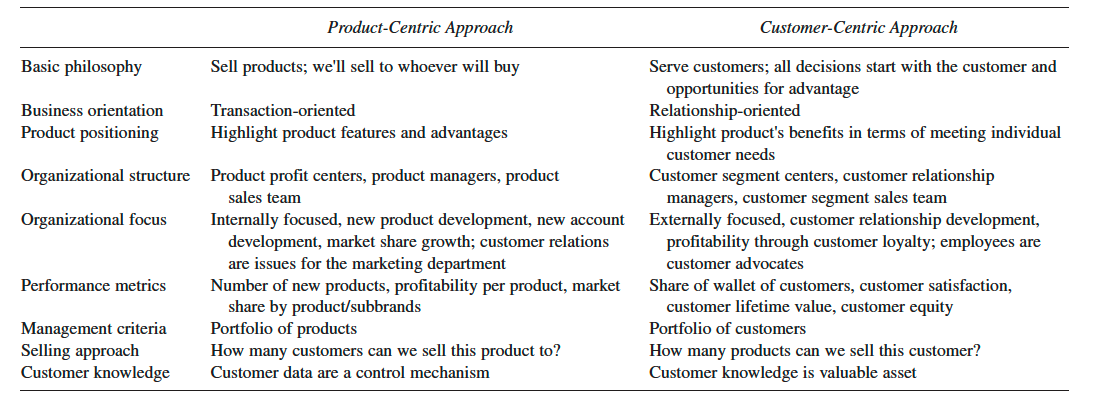
\includegraphics[scale=2, width=\textwidth]{dippa/images/ProductVsCustomer.png}
    \caption{Differencies in product-centric and customer-centric approaches by \textcite{PathToCustomerCentricity:2006}.}
    \label{fig:productvscustomer}
  \end{center}
\end{figure}

Being closer with the client means that the company have customized their offerings to individual customers. This is reported to happen for example by collecting information about their customers in order to understand buying patterns and through this the company has been able to influence the future purchase. To do so, the company also needs to view the problems from the perspective of the client and not through their own products. When company does this, they focus on satisfying customer needs and solving their problems and thus it can be said that they sell solutions. \parencite{Parniangtong:2017}

The value of trust and intimacy go hand in hand. A company must gain trust from the customers in order to maintain the relationship. When trust is earned, the goal is to create value through customer intimacy because companies want that making business with them is easy. To do so, company must show to the customer that they care about them, value their business and are aware of their needs as individual and unique customers. \parencite{Parniangtong:2017}

To gain the long-term profits from a customer-centric view, the company need to succeed in the following areas: customer acquisition, customer retention and customer development. Customer acquisition aims to get highly committed customers to be as advocates for the company by helping to look for new customers, increase the amount referrals and understand the cost as well as the value of new customer acquisition. The goal of customer retention is to lengthen the relationships between the company and the best customers as well as to lower the cost of maintaining such relationships. Lastly, customer development strives to develop customers in the direction where they would buy more products or services from the company. \parencite{Fader:2012}

\subsection{Customer Journey Maps}

Based on \textcite{Kalbach:2016} operational efficiency of a company is thought as more important than their customer 
satisfaction. To turn this situation around, alignment diagrams can be used to help organizations to think how their business fit to the lives of customers. Alignment diagrams present the interactions between a customer and an organization in a storytelling way. Additionally, the diagrams offer a way to show both sides of value creation since they help organizations to visualize the strategy as well as they help to design experiences. \parencite{Kalbach:2016}

Alignment diagrams are beneficial because they build empathy, provide a big picture, break silos in organizations, help focusing and point where improvements and innovations can be made. Understanding better people's thoughts and feelings through alignment diagrams build empathy which allows an organization to learn about their customers and real-world human conditions. With the alignment diagrams it is possible to share the understanding and provide a big picture in organizations because the actions become more consistent and the decision making is influenced by the diagrams. \parencite{Kalbach:2016}

Because the alignment diagrams allows to map the customer experiences across different organization departments, it is possible to break down silos. In addition they help organizations to focus because alignment diagrams match the outward-facing activities with inward-facing activities. Lastly, the alignment diagrams reveal opportunities for improvements and growth because the presentation of the information allows it to be understood without middlemen. \parencite{Kalbach:2016}

According to \textcite{Kalbach:2016} the value in mapping experiences becomes from the fact that it allows to discover innovative ways to make interactions better. Moreover, the whole design of the system is then easier to make coherent.

Customer journey maps CJMs are type of alignment diagrams and \textcite{Kalbach:2016} defines customer journey maps to be visualizations about a customer's experiences and usually they illustrate how customers make a choice for example a decision to buy a service. So, customer journey maps present the steps the customers take while engaging with the company through different touchpoints \parencite{Richardson:2010}.

More precisely, CJM's present the interactions in a chronological way including for example customer's actions, thoughts, feelings and pain points. From the organizational view point the CJM's present the roles and departments who are part of creating the experience for the customer. \parencite{Kalbach:2016}

Nowadays, multi-channel shopping has become a standard in the consumer decision-making process because of mobile technologies and social media. 

Customer Buying Behavior Process Model
path-to-purchase modeling
f customer decision processes and
experience when buying products



\chapter{Methodology}
\label{chapter:methods}

The research was a qualitative study which followed design science research. This chapter introduces the methodology and methods as well as tools used in the study. Finally, the research implementation is presented.

\section{Design Science Research Methodology}
\label{section:overview}

\textcite{Aken:2014} describes \emph{Design Science Research DSR} to be a problem solving research strategy which should produce actionable knowledge in order to address types of field problems. The knowledge is used as a means, not as an end which means that the knowledge can be applied in a direct way to realize the desired outcomes. This is done by developing artefacts which should solve the problem experienced by people \parencite{Johannesson:2014}. As stated above, the design science research is driven by the field problems rather than knowledge problems, meaning that the problem is defined in the real world situation by stakeholders. 

According to \textcite{Johannesson:2014} the designed artefact can be a construct, method, model or instantiation. Constructs help to formulate problems and answers for them, meaning that they are definitional knowledge. Definitional knowledge means that with them it is possible to speak statements about the world rather than make the statements about the world. Methods define guidelines and processes which are meant to solve problems and achieve goals. Additionally, methods can be informal and be used as best practices. Models are used to represent possible solutions for a practical problem which means that they can be used to define the construction of the artefact. Lastly, instantiations are systems which are used in practice.

The design science research aims to produce a solution concept which would then be used to solve the field problem. This solution concept is used in the context by a design proposition. Design proposition can be formulated using CIMO-logic, which stands for this problem-in-\emph{C}ontext, it is useful to use this \emph{I}ntervention to produce through these \emph{M}echanisms this \emph{O}utcomes.

DSR-project has three parts \begin{enumerate}
\item An explanatory part which consist of analyzing and framing of the chosen type of field problem.
\item A design part when an intervention is designed and tested in an iterative way.
\item A testing part where the final version of the intervention is tested. \parencite{Aken:2014}
\end{enumerate}

\textcite{Peffers:2007} created a methodological framework for doing design science which complements and gives more precise activities for doing a DSR-project. This methodological framework, \emph{design science research methodology}, is divided into six different phases. The first activity is \emph{problem identification and motivation} where the specific research problem and justification of the value of a solution is defined. \emph{Defining the objectives for a solution} is the second activity where the objectives of a solution are inferred from the problem definition.

Next, the artifact which can be model, method, instantiation or construct is \emph{designed and developed}. Then the artifact is used to \emph{demonstrate} how it can be used to solve the identified problem. The artifact is \emph{evaluated} on how well it supports solving the research problem. This is done by comparing the objectives of a solution to the actual observed and measured results from the demonstration. Finally, the knowledge should be communicated to researchers.

\textcite{Salvatore:1995} state that design science aims to create things to serve human purposes. As stated earlier, the four types of products that design science aims to produce are constructs, models, methods and implementations. Additionally, design scientists develop ways to perform goal-directed activities which are innovative and valuable. The purpose of this study is to increase the understanding about housing company decision making as well as improve the current sales process. Thus, it is justified to use design science research since, as mentioned, the purpose of design science is to produce actionable knowledge to address the identified problems.

\section{Semi-structured Thematic Interview}
\label{section:interview-info}

According to \textcite{Wilson:2013} a semi-structured interview combines open-ended exploration with predefined questions and it usually follows a interview guide which offers a frame to conduct such interviews. The interview guide consists of an introduction to the topic and the purpose of the interview, a list of topics and predefined questions to ask, probs and promts and comments to end the interview.

The semi-structured interviews are done in a conversational manner even though there can be predetermined questions. It is a good method in order to investigate behaviours, opinions and emotions as well as to gather experiences. It provides a way to get more details about a topic where there is already some knowledge, but it lacks a deeper understanding. For the interviewee the semi-structured interview allows to focus on topics which they feel more important. In addition compared to the structured interview, the answers are open and not yes or no type of answers. \parencite{Cliffod:2010,Wilson:2013}

According to \textcite{HH:2001} semi-structured thematic interview is based on the focused interview which was published in a book \emph{The Focused Interview} written by Merton, Fiske and Kendall. The most relevant aspect of thematic interview is that the interview is going forward based on the themes rather than detailed questions so, it provides a framework for discussion. This allows the interviewees to answer more freely with their own wordings in order to bring their experiences to the center of attention and thus for the interviewer it is possible to collect insights about what people do and think \parencite{Cliffod:2010}.

As stated above, semi-structured interview as well as thematic interview have many strengths considering the flexibility, gathering experiences and the comparison between the interviews. However, it is important to be aware of that the interviewer do not put words into the interviewee's mouth or guide the discussion into particular answer during the interview. Since, the semi-structured interview is flexible, it is crucial for the interviewer to be also consistent in order to make comparisons between the interviews. \parencite{Wilson:2013}

Since, the purpose of first research question was to find out what affects the purchasing decision making in the housing board it was justified to conduct semi-structured thematic interviews in order to discover the real feelings and operations inside the board. The interview was chosen because it provides a way to get deeper understanding by collecting detailed information \parencite{Johannesson:2014}. In addition the semi-structured interview allows the discussion to flow freely and the interviewees were able to describe the situations more broadly compared to structured interview.

\section{Lean Service Creation}

It is stated by \textcite{LSC} that \emph{Lean Service Creation LSC} helps bringing customer centricity into work, workflow and internal process development. Additionally, the LSC helps to communicate ideas and it forms a shared language. In practice, LSC is a set of tools which help multidisciplinary teams to create new services and products. It is based on Lean Startup, Agile methods and Design thinking. LSC offers canvases which outline the relevant phases in a service creation process and it is at the hands of the user to decide in which order the canvases should be used. According to the creators of LSC, the mindset and practices are the foundation for successful service creation.

Since, the actual study was conducted as a service design project it was justified to use some tool set which would help the research process. Lean Service Creation was chosen because it was familiar for the researcher and it also fit the process of the design science research. Moreover, LSC helps to think more about the customers and thus, the usage will increase the customer centricity. 


\section{Research Implementation}
\label{section:research-implementation}

The Next chapters describes how the actual research was done phase by phase. The phases of the design science research methodology together with activities done during the study are presented in the The Figure~\ref{fig:dsrm-implementation}.

\begin{figure}[ht]
  \begin{center}
    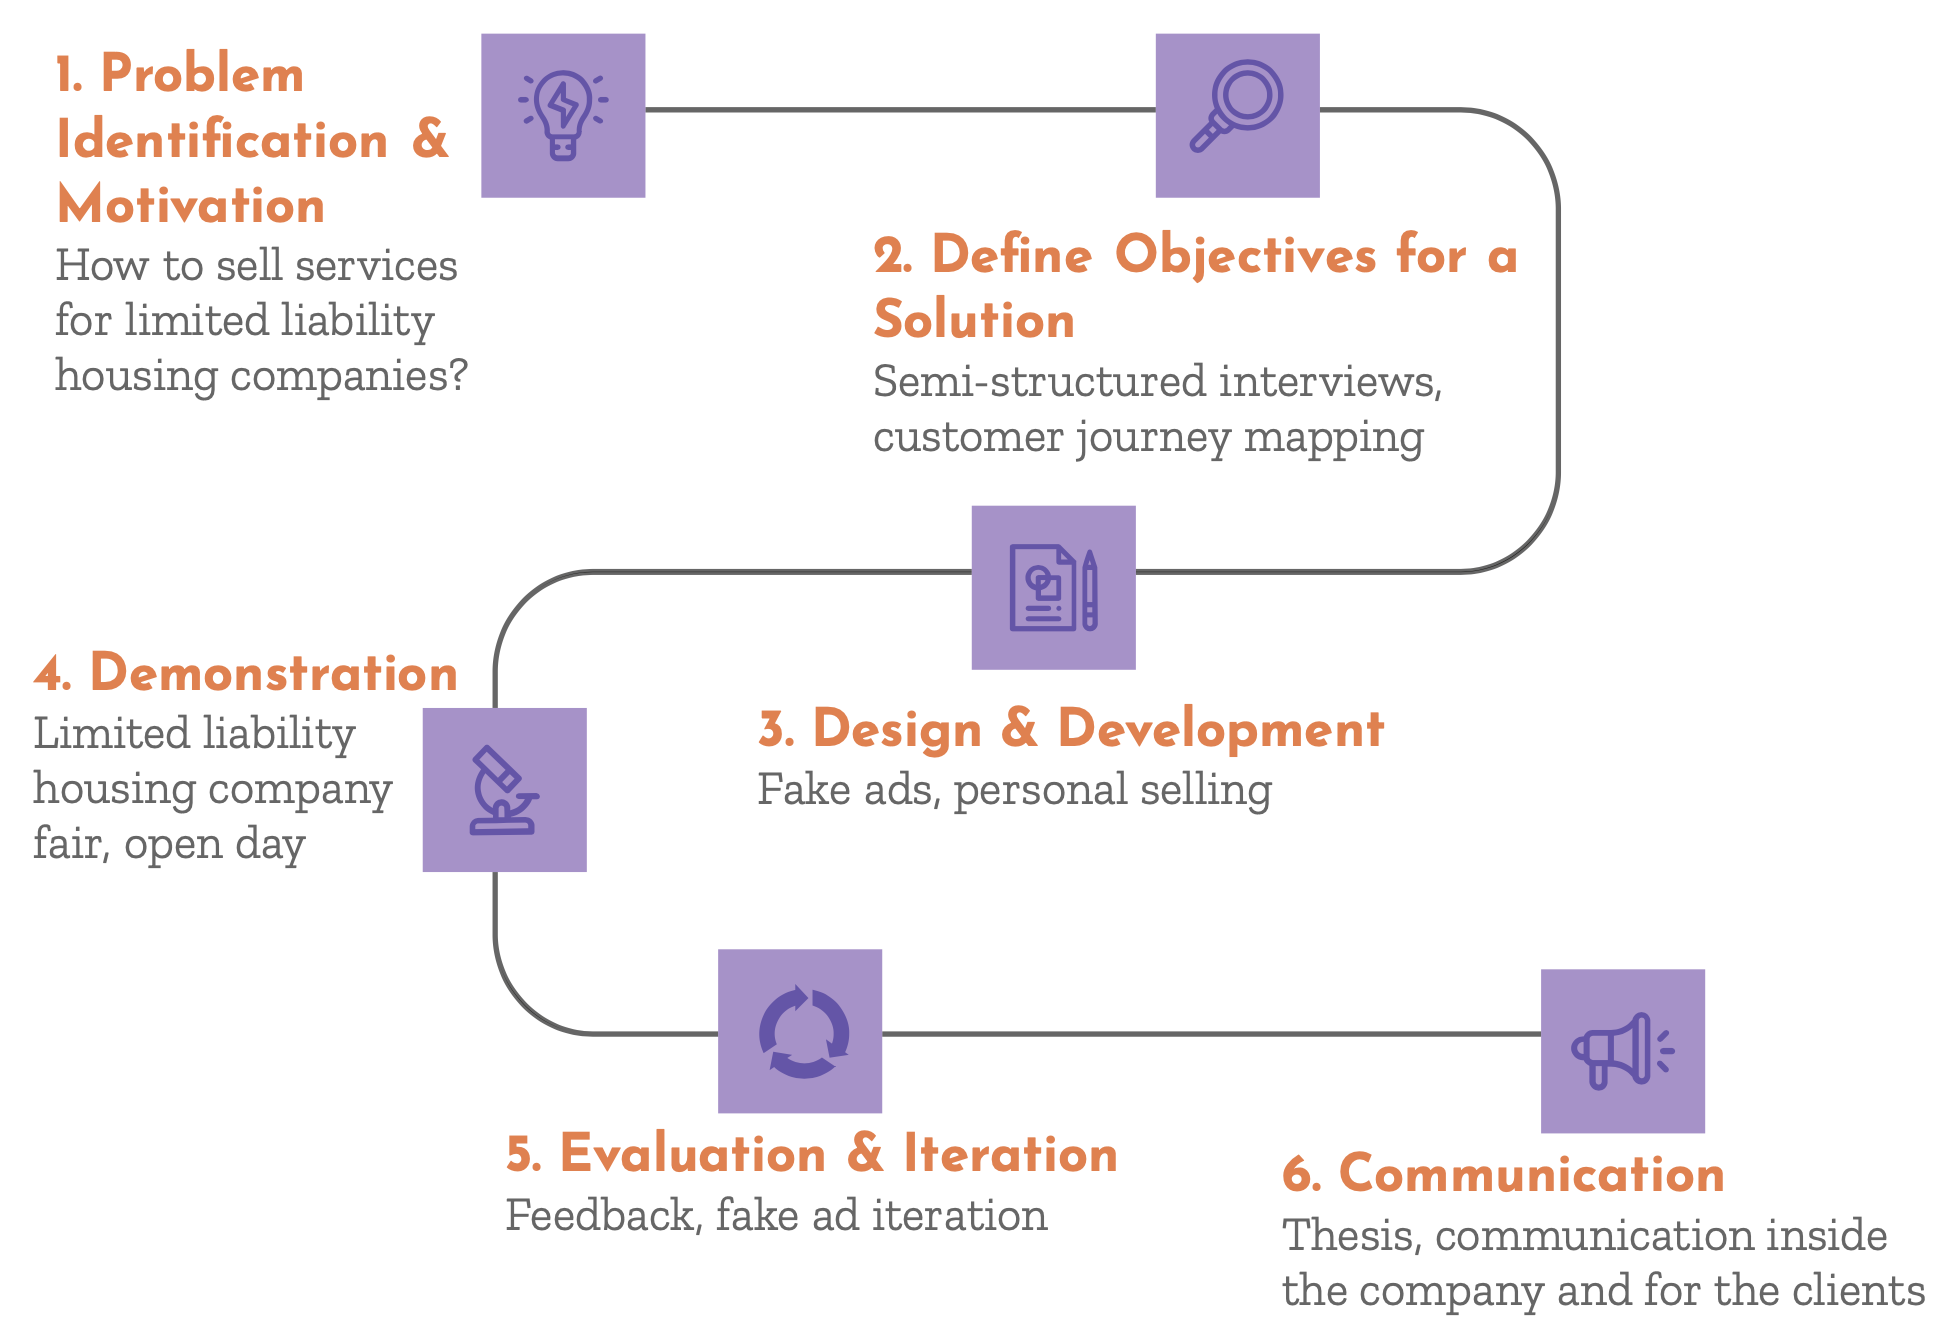
\includegraphics[width=\textwidth]{dippa/images/dsrm-implementation.png}
    \caption{The research process and the conducted activities.}
    \label{fig:dsrm-implementation}
  \end{center}
\end{figure}

\subsection{Activity 1: Problem Identification and Motivation}

Based on the DSRM process the study started with the first activity, problem identification and motivation. The case company was in the situation where they needed to expand their sales, and in order to grow bigger in Finland, they needed housing companies as clients. The problem in acquiring them as clients was that the case company had not done business to customer selling much and they needed to gain more understanding about how the housing company works and makes decisions. This problem then lead to the first research question \emph{What affects the purchase decision making in a limited liability housing companies}.

In addition to understanding the decision making in housing companies, it was important to discover a sales process which would take into account the case company's and partners viewpoints as well as the end-customers' viewpoints in order to make acquiring housing companies as clients easier, faster and unified. From this problem the second research question was formed as \emph{How to improve current sales process with the knowledge of limited liability housing company’s decision making process?}

Literature review was conducted in the Chapter 2 and it included the relevant background research about housing company, energy industry in Finland, decision making process and customer centricity. housing companies were studied in order to understand the operation and the legal backgrounds of its actions. Energy industry in Finland were researched in order to understand the current state and future opportunities. In order to design some improvements for the sales process it was crucial to understand how humans make purchasing decisions. Lastly, the concept and benefits of customer centricity was presented.

In order to understand the motivation and the problems of energy companies, the researcher participated in several partner meetings and observed them. In addition the researcher did observation at the workplace and that knowledge was applied in several occasions. The researcher also used few canvases from the LSC in order to make communication easier with the relevant stakeholders and to make the discussed topics more tangible.

\subsection{Activity 2: Defining Objectives for a Solution}

\subsubsection*{Data Gathering}

The second activity of a DSRM, defining objectives for a solution was done by conducting semi-structured interviews with the board members of housing companies. To gain broader understanding the researcher did six interviews with people of different age and their experience level in the board varied from one year to almost twenty years. Additionally, the people were either chairpersons or members of the board. The interviews that lasted from 40 to 80 minutes and they were conducted as face to face meetings and recorded in order to listen and analyze them afterwards. The relevant information related to the interviewees role, experience in the board, age, occupation and the duration of the interviews are presented in the Table~\ref{table:interviewtb}.

The thematic interview was divided into four categories in order to answer the \emph{RQ1: What affects the purchase decision making in a private housing company board}. These themes were defined in order to gain insights about why people go to board, how the board operates in practice and what kind of things influence their work. The themes covered in the interviews were as follow: being part of the board, decision making in the board, influences on housing company operations and energy efficiency. The first theme dealt with reasons why the interviewees were members of the board and their feelings about their work in the board in general. Second theme covered the process of decision making with examples of previously made investment decisions and the role of money in them. Third theme concentrated to learn about influences that affects the operations of the board as well as who the board trust and where they find information related to services provided for housing companies. Lastly the energy efficiency topic discovered how well are energy efficiency topics understood in the boards of the housing companies and the importance of it.

\begin{table}
\begin{tabular}{|p{2.3cm}|p{2.8cm}|p{1.8cm}|p{2.7cm}|p{1.9cm}|} 
% Alignment of sells: l=left, c=center, r=right. 
% If you want wrapping lines, use p{width} exact cell widths.
% If you want vertical lines between columns, write | above between the letters
% Horizontal lines are generated with the \hline command:
\hline % The line on top of the table
\textbf{Role} & \raggedright\textbf{Experience in the board} & \textbf{Age} & \textbf{Occupation} & \textbf{Duration} \\ 
\hline 
% Place a & between the columns
% In the end of the line, use two backslashes \\ to break the line,
% then place a \hline to make a horizontal line below the row 
Member & 17 years & 59 years & Director & 40 mins \\ 
\hline
Member & 11 years & 36 years & Energy expert & 80 mins \\  
\hline
Chairperson & 5 years & 30 years & IT-consultant & 80 mins \\
\hline
Chairperson & 10 years & 76 years & retired & 60 mins \\
\hline
Chairperson & 19 years & 70 years & retired & 75 mins \\
\hline
Chairperson & 1 year & 31 years & Electronics engineer & 45 mins \\
\hline
\end{tabular} % for really simple tables, you can just use tabular
% You can place the caption either below (like here) or above the table
\caption{Information about the interviewees.}
% Place the label just after the caption to make the link work
\label{table:interviewtb}
\end{table} % table makes a floating object with a title

\subsubsection*{Data Analysis of the Interviews}

\textbf{Analyzing of the interviews was done by listening the interviews again and taking notes of relevant points and afterwards clustering them into categories.} The researcher divided the notes based on the LSC user insight canvas since it was familiar way for the researcher to help analyzing the interviews. The user insight canvas categorizes the notes for user needs and problems, what surprised the researcher and what the user thinks and feels.

According to \textcite{HH:2001} the researcher knows the interview material so well that it is easy for her to recognize the themes covered and make notes about dialogue when needed. Thus, in this study the researcher did not transcribe the interviews since there were only six interviews to be analyzed and the researched conducted the interviews alone.

\subsubsection*{Observing the Energy Industry}

\textbf{In addition to the interviews}, the researcher participated many meetings where the energy company was present in order to \textbf{observe} and gain more insights about the industry. From the meetings, the researcher gained understanding on how well do the energy companies understand the housing companies as their customers and how much they have communication with them. Additionally, the researcher learned about the drivers to have case company's solution as part of the company's service offering. To understand more about the energy company the researcher and the team categorized energy companies into three different segments based on their team size, speed to take things forward and willingness to proceed with service business.

\subsubsection*{Customer Journey Mapping}

To design a better way and providing guidance on how to acquire customers it was first necessary to go through the current customer journey as described in the chapter 2.4.1. For this, the researcher used LSC canvas for visualizing customer engagement. The canvas helps to list all the steps from rising customer awareness, engagement, purchase, use, use more and advocate combined with the touchpoints. By listing also the enablers and problems it was easier to discover problems.

The canvas was filled with one energy company and it was also complemented with the knowledge gained from other meetings with energy companies. From this work it was decided to focus on the first three steps in customer engagement canvas which were awareness, engagement and purchase because it was identified that those are the biggest bottlenecks. Additionally the case company's product is sold by the partners and they can sell the service in which form the want but they lack the knowledge about how to actually approach the housing companies.

\subsection{Activity 3: Design and Develop}

The third activity in design science research is design and develop and the purpose is to design an artefact which addresses the stated problem and fulfills the defined objectives \parencite{Johannesson:2014}. So, to answer the second research question \emph{How to improve current sales process with the knowledge of limited liability housing company’s decision making process?} the researcher together with the team conducted few tests to gain insights which would then work as a base for improvement suggestions. The Figure~\ref{fig:experiments} presents the two tests which were done related to the pricing model and personal selling as well as consulting.

\begin{figure}[ht]
  \begin{center}
    % here the width of the figure is set to 9 cm
    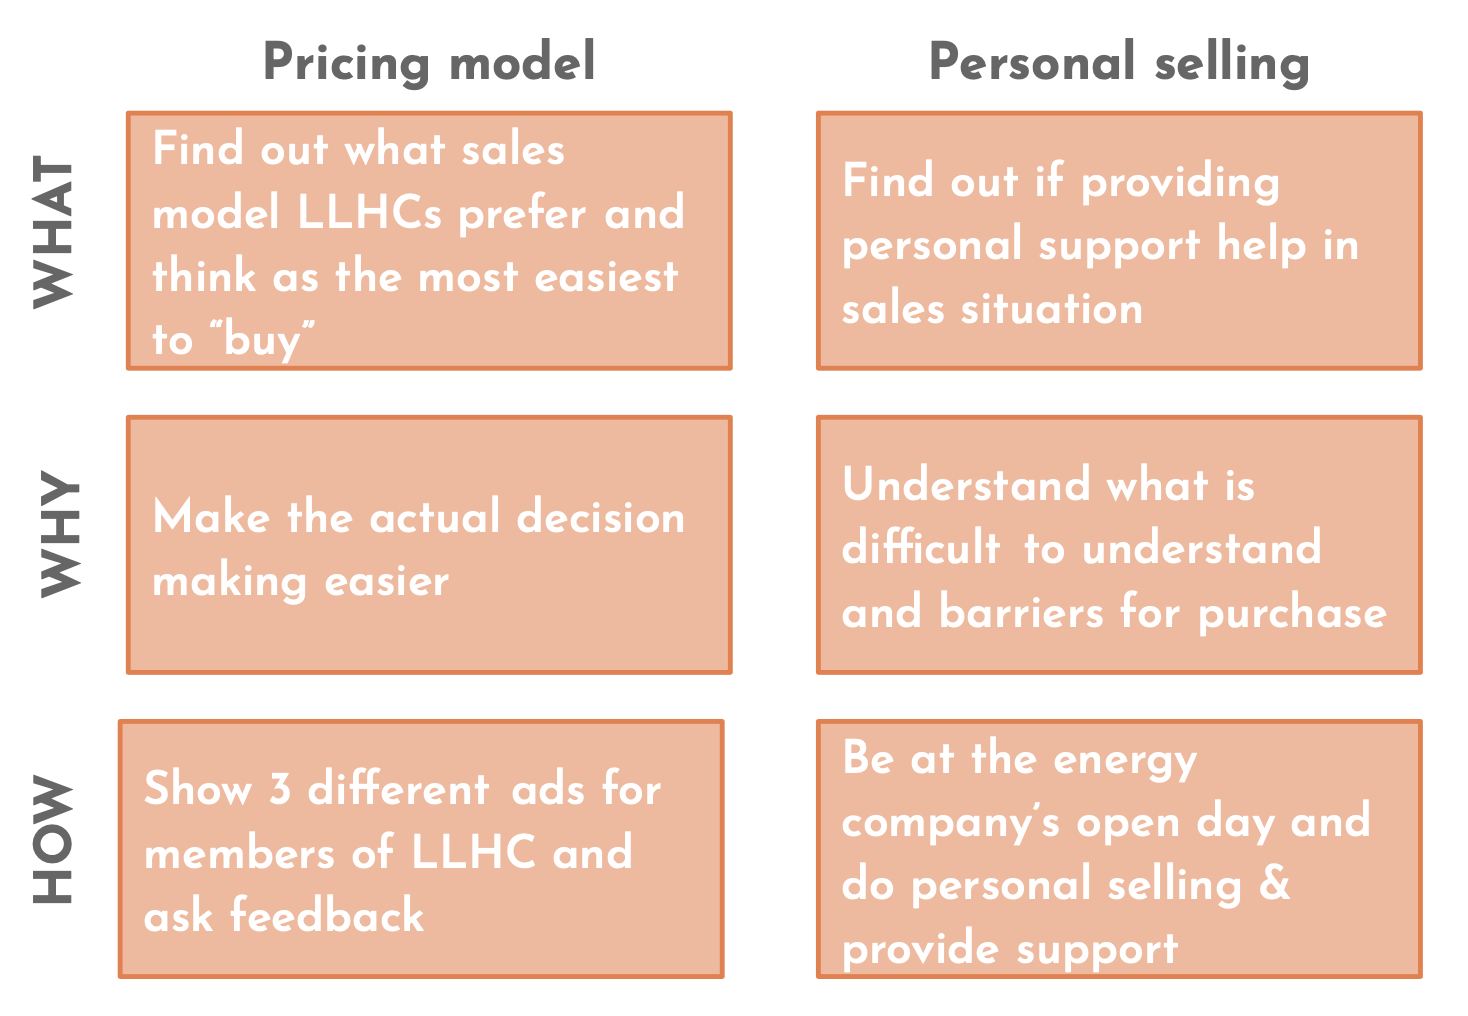
\includegraphics[width=\textwidth]{dippa/images/experiments.png}
    \caption{Conducted experiments.}
    \label{fig:experiments}
  \end{center}
\end{figure}

\subsubsection*{Fake Ads}

Pricing model had risen as a big concern among the case company and the energy companies since they did not know what model would work best for the housing company. In addition, the partner company had a service already in the market but they were struggling with the pricing model. So, to find out which model the housing boards would prefer and why, the researcher and the team designed three different fake ads which were all looking the same but the pricing model was different in each of the ads. Additionally, the communication of the fake ads were following the \emph{start with why} philosophy as described previously in the chapter 2.3.

The fake ads had three different kinds of pricing models which were as follows:
\begin{itemize}
	% You can use this command to set the items in the list closer to each other
	% (ITEM SEParation, the vertical space between the list items) 
	\setlength{\itemsep}{2pt}
	\item Investment plus a monthly service fee,
	\item A monthly service fee.
	\item A monthly service fee which is covered by the saved energy fees.
\end{itemize}

\subsubsection*{Personal Selling with Personalized Offers}

From the interviews done with the housing companies, it was clear that they need consulting and help when the offered service is new to them. Additionally, clear communication, making things as simple as possible and providing support are important when being in contact with them. With this in mind the the researcher participated one open day organized by an energy company in Finland. There the researcher was able to provide support and answer the questions about the service. Moreover the researcher was able to do personal selling. Lastly, to improve the engagement and to help purchase decision making easier the researcher and the team made personalized offers, which were available in the open day, by adding the potential amount of saving for the housing companies. This was done in order to reduce the pain and increase the net value as presented in the chapter 2.3.

\subsection{Activity 4: Demonstrate}

\subsubsection*{Limited Liability Housing Company Fair}
The three different fake ads designed were tested in the housing company fair which was aimed for the board members of housing companies. The specific fair was chosen because the main audience there were purely the board members because the idea behind the fair is to present services and products for the housing companies. The fake ad testing was done together with one energy company who is also partner of the case company.

The ads were shown for 12 people and asked to read and comment the ads. The testing was done mainly in pairs which allowed the other to present the ads and the other to make notes about the test session. The team approached people in the fair and asked if they would be willing to give opinions about the ads. The ads were given for the volunteers and after a moment the people needed to choose one of the ads which had the pricing model that they prefer the most. The team asked reasons behind the choice and also feedback about the ads in order to find out improvement ideas.

\subsubsection*{Energy Company's Open Day}

Since, it was clear from the interviews that lack of expertise in real estate or building industry are typical issues in housing companies the researcher took part in an energy company's open day in eastern Finland in order to do personal selling. The purpose was to be there in person and to promote their service which is built on top of the case company's technology. In the open day the researcher had personalized offers for the area's housing companies.  The offers also included improvements from the previous test done in the housing company fair.

The offers all had the same monthly cost but in the offer it was also stated how much is the predicted saving if they would have the service in use. The researcher was able to contact the members of housing companies in person, answer the questions immediately and also to collect contact information from interested buyers.

The researcher was able to discuss with three members of housing company, the rest of the people were mainly living in detached houses. All of them received an offer and their contact information was collected for the energy company to be in contact with them afterwards.

\subsection{Activity 5: Evaluate and Iterate}

In the second to last activity of DSRM the designed artefact is evaluated to see how well it solve the initial problem and fulfil the set requirements. To answer the RQ1 the researcher analyzed the interviews and formed requirements which were then used to form guidance of how the improved sales process should go. Additionally, the interview result can be used as guidance since they increase the understanding of the operation of housing company.

To answer the RQ2, the researcher together with team did different test to gain insights about what works and what not in acquiring housing companies as clients. The test were evaluated also from the business perspective and objectives.

Since, the purpose of this study was to gain more knowledge about the housing companies and to form suggestions the results can also be used in order to find out future research areas.

Iteration was not possible to do for the whole process because of the research time span. However, the ads were improved after test sessions and the insights gained from the test sessions were always further used in the next sessions as well as daily work. In addition, the researcher describe the future research ares and recommendations of what should be done next.

\subsection{Activity 6: Communicate}

The last activity of the DSRM consist of communicating the results of the study and this is done through this thesis. In addition, the results are presented in the case company as well as for the case company's energy company partners if possible.
 
\chapter{Results}
\label{chapter:results}

In this chapter the results of the study will be presented. First the limited liability housing company board member interview results are presented. Then the researcher presents the results gained from customer journey mapping which was done together with energy company and. Lastly, the researcher presents the results from the prototypes and tests conducted during the research. 

\section{Limited Liability Housing Company Board Member Interview Results}
\label{section:interviews}
In this chapter the results of the interviews are discussed and presented by the themes found in the analyzing. The themes are motivation of the board, role of the deputy landlord, overall decision making in a housing company, identified board types and awareness of energy efficiency.

\subsection{Motivation of the Board}

Motivation of the board was discovered to be the biggest factor affecting the actions of a board of the housing company. Based on the interviews, the reasons why people are part of the board and what kind of people they are affects the motivation and operation of the board.

\subsubsection*{Reasons to be in the Board}

The reasons why people are in the board of housing companies varies and it is not the same for everyone but usually the reasons are overlapping and connected to each other. The following themes were identified as reasons to be part of the board:
\begin{itemize}
	% You can use this command to set the items in the list closer to each other
	% (ITEM SEParation, the vertical space between the list items) 
	\setlength{\itemsep}{1pt}
	\item Take care of the value of the investment.
	\item Make sure that things are done correctly.
	\item Personality and experience of the people.
	\item Other people persuade.
	\item Desire to make housing company better and modern.
\end{itemize}

The main reason found out was that the members of the board want to take care of the investment's value they have made when buying the apartment. This reason is based on the fact that living in a detached house is basically the same thing as living in an apartment house and both of them needs maintenance in the same way.

\begin{displayquote}
\textit{I had a bigger risk to loose my money if I didn't go there (to the board). I wanted to make sure that the traditional pipe repair will come and that it will get done.} --- interviewee
\end{displayquote}

\begin{displayquote}
\textit{I also do not understand what is so difficult that people do not want (to go to the board). I find it really important that it is my property and it needs to be treated well. -- The apartment building requires care as well as a detached house.} --- interviewee
\end{displayquote}

Taking care of the investment's value is connected to the fact where the people want to make sure that the things are done with care and correctly. This can be the case even though there is no investment made on behalf of the board member. One interviewee who did not live in the building was part of the board because of his relative was living in the building and he wanted to make sure that the good living conditions were guaranteed and that the things run smoothly in the housing company.

\subsubsection*{Background and Personality of the People}

From the interviews it was also clear that personality and background of the people play a role in why people go to the board. Some of the interviewees felt responsibility to be in the board since no one else had volunteered. In some cases this responsibility is also connected to the need of taking care of the investment's value. Another big factor was found out to be the people's background in work context. Three of the interviewees had work experience in some sort of real estate field and thus had interest also in housing company's operations. Because of the work experience, they were usually also driving topics and projects which are related to their own work field.

\begin{displayquote}
\textit{Those needed to be dug, that I was there also waiting for awhile. And I left there with the thought that I will not go to the board and there I am now. And it seems like there is no way to get rid of it.} --- interviewee
\end{displayquote}

In some cases there had been difficulties to get people to the board. In some cases the reason why they still were part of the board was that nobody else had been voluntary to replace them and thus they felt obligated to continue. However, it would be wrong to simply state that they are forced to continue, rather, they are by character that kind of people who take more responsibility when nobody else is willing.

Another fact which was identified to be a reason why people go to the board was that other people had persuaded them. It means the person might not have gone to the board without someone else persuading them or promoting them for the position. In one situation another person had stated that they will not run for the chairperson position if the interviewee would have not agreed to go for the board.

Finally people's desire to make housing company better and modern was identified influencing the reasons why people are in the board. In this situation the work experience of the board member had a big role. If a board member had expertise in the area which could be applied e.g. for building maintenance, it affects the willingness to be in the board and drive projects related to the expertise the member has. 

\subsubsection*{Elements of Motivation}

The reasons why people are in the board form a base for the board's motivation, activity and actions. In addition motivation is related to the time allocated for the board work, some meet every month to discuss housing company related matters and some meet only once a year when it is compulsory.  On top of it, the motivation of the board consists of the following elements:
\begin{itemize}

	\setlength{\itemsep}{1pt}
	\item Spirit inside the board
	\item Initiative
	\item Expertise inside the board
	\item Trust inside the board and between the board and deputy landlord
\end{itemize}

Spirit inside the board affects the working environment and the pro-activeness of the board. If the spirit is good inside the board, the co-operation naturally works better. A good spirit creates a foundation for the people to discuss about the topics and ask questions. In addition the spirit is also related to having meetings, one interviewee stated that having meetings is not always required if things can be also agreed and discussed via email.

The interviews revealed that initiative of the board is a big factor in driving the actions. Moreover initiative is highly affected by the people especially if there is a lot of expertise in the board. The more expertise there were on the board, the more pro-actively the board was operating.  One of the key findings related this topic was that if there was people who have expertise in the real estate field in the board, the housing company is more advanced in doing actions which make the building so to speak better rather than maintaining it as it is. Moreover, it can be stated based on the interviews that even one person who has work experience in real estate is enough to drive the housing company operations in that specific area. In contrast, if the board did not have experienced people the actions were mostly done to keep the building as it is and fixing some noted faults.

Trust was highlighted as an important aspect of the work. It was important that the board members trust each other to do the tasks assigned in order to take care of the running things. In addition the trust towards deputy landlord was seen as a key topic. The deputy landlord takes care of the financial of the private housing company and execute the given tasks, if there is no trust the whole operation of the housing company would not happen.

\subsection{Role of the Deputy Landlord}

\begin{displayquote}
\textit{We went with the deputy landlord's saying: ‘this is how it is usually done’.} --- interviewee
\end{displayquote}

In all of the interview cases deputy landlord was seen as an expert who has the education and skills to be in charge of the housing company. However, most of the interviewees stated that majority of the deputy landlords are not meeting the expectations that the housing companies have nowadays. In addition, deputy landlords are seen as service provider but the problem is that the deputy landlords have not understood it yet. In a situation where the deputy landlords are still in a way operating in the past, a big responsibility to drive the housing company's matters is in the hands of the board and when the board do not have motivation or skills to do it, only compulsory tasks get done.

\begin{displayquote}
\textit{Deputy landlords do not understand that they are a service that we buy.} --- interviewee
\end{displayquote}

\begin{displayquote}
\textit{Deputy landlord is not an expert in technology development.} --- interviewee
\end{displayquote}

Traditionally deputy landlords keep track and report the financial as well as take care of the practicalities. However, there is an increasingly need of deputy landlords who are on top of new technological services and products which could help the work of the board as well as the maintenance of the building. Many interviewees stated that they do not feel it is their job or responsibility to improve or find services which would benefit the operation and building maintenance. The reasoning behind this statement was that the members of the board do not feel like they are the experts nor have the education to be in that position. Exception to this is when the board members have some expertise, however in those situation they also wish deputy landlord to be on top of things. Even though deputy landlord is seen as the professional, the board members highlighted their own responsibility to find out and learn about the topics discussed in the meetings in order to do justified decisions.

\begin{displayquote}
\textit{A lot of money would be saved in this country if we had good
and active deputy landlords in every place. It is good thing if the
housing board is active but it is the job of the deputy landlord.} --- interviewee
\end{displayquote}

In all of the cases the interviewees told they have a lot of discussions with the deputy landlord. Trust between the board and the deputy landlord was emphasized to be one of the key things in the housing company operations. Without trust the housing company could not even operate.

\subsection{Decision Making in a Limited Liability Housing Company}

The research was first lead with an assumption that the decision making in the housing company is difficult. However, all of the interviewees stated that the decision making itself is not difficult. The people who are in the board does not necessarily have the competence and understanding of the topic discussed which makes the decision making difficult. Key learning from easiness of decision making was that the topic needs to be openly discussed and everyone needs to understand what it means. Problems arise when someone does not understand and is afraid to ask more. In addition the board needs to build trust between each other and between the shareholders. One interviewee pointed out that they actually do not vote on anything in the general meeting, but they present the projects or topics which will start for the general meeting.

\subsubsection*{Drivers for Actions}

The role of the deputy landlord in the decision making is not that significant. The deputy landlord can introduce new things for the board but then the conversation starts and the decision can be different than what the deputy landlord originally suggested. However, the board always listens the suggestions of the deputy landlord and they trust their expertise if it has not been compromised. After the deputy landlord has suggested something, the board usually discusses about it and then decides on it and the decision can also be the opposite of what the deputy landlord had suggested.

\begin{displayquote}
\textit{Because of built trust we have a strong initiative and we can basically decide between the board to start proceeding something. It is then well justified in a general meeting and we get a so-called blessing for it.} --- interviewee
\end{displayquote}

The interviewed people did not feel pressure of the work in the board or about the decisions they have made. The decision making is highly affected and influenced by the thought where all things done need to consider the residents of the building. Key value in the decision making is to do such things which will provide good living conditions for all residents. If a strategy is made in the housing company it is used to backup the decisions. Without the strategy it is really hard to justify decision or projects which should be done in the building.

Another factor influencing the actions and maintenance decisions of the building is the service providers and sales men, even though their influence is not that remarkable. The chairperson receives a magazine which is made especially for the housing board. In addition, the chairperson receives offers and calls from various service providers who are offering their products and services for housing companies. Identified problem with these contacts were that the chairpersons might not have the competence to think the relevancy of the provided service in their specific case. It is then heavily on the hands of the chairperson to present the received offers to other board members and deputy landlord. If the chairperson is not that interested in them, it is likely that the offers and magazine will just be forgotten.

\subsubsection*{Money versus Living Conditions}

Money was stated to be influencing the decisions made in the board but not as the most important aspect. The investment decision making was described to go as follows: First the idea for renovations comes either from some of the resident, deputy landlord or it is stated in the strategy. Then it is discussed in the board and decision is made to proceed with the project and usually at that time the deputy landlord is asked to send bids if the board do not want to do it themselves. The offers are handled inside the board and one of them is chosen. If the decision can be done without the general meeting, the project starts and the deputy landlord as well as the members of the board usually keep an eye on how the project proceeds.

\begin{displayquote}
\textit{There is a big responsibility with the board, to think the whole at all times. That sometimes the most reasonable decision is not the best. Because you need to think about all the people who are living in the building, so that they can live there and in which order to do (renovations) so that the cost burden does not get too big.} --- interviewee
\end{displayquote}

\begin{displayquote}
\textit{Saving is the worst thing you can do in a private housing company.} --- interviewee
\end{displayquote}

The key learning from decision making was that the money is not the key driver in decisions as mentioned above. However, the interviewees stated that if there are a lot of people who rents the apartment and do not live there by themselves, the decisions might be driven more from the perspective of saving money. But in the situation where most of the people who own the apartments are living there too, the decisions are done more from the perspective of living conditions but still in a cost-effective way.

\begin{displayquote}
\textit{You have to think economically, but still with a heart.} --- interviewee
\end{displayquote}

\subsection{Different Board Types}

From the interviews two themes rose as the most important responsibilities of the housing board. These were taking care of the structures and providing good living conditions for everyone. It was important for the board members to observe the building conditions in order to avoid big surprises which would be costly for the housing company. This means the renovations should be done in advance and in smaller peaces in order to lower the costs and the renovation burden.   

\begin{displayquote}
\textit{It is cheaper for every one if things are taken care of. That you are not like a fire department that you put out the fire when it has already happened. Rather you should be up to date and see what is the situation at all times.} --- interviewee
\end{displayquote}

\begin{displayquote}
\textit{If you save too much, the state of the building weakens. It will just deteriorate if nobody does anything. And nobody will do anything for free.} --- interviewee
\end{displayquote}

As stated before there are differences in the housing companies related to how active the board is in driving various projects. Two different mindset, making building better or keeping it at the same status, are driving the actions based on the responsibilities. Running the housing company with the mindset to keep it as it is covers mainly the actions related to structures of the building. When it comes to the enhancing living comfort, the mindset can be either keeping it at the same or upgrading. Upgrading the living conditions usually means renovations or actions which are considered as \emph{nice to haves} such as redoing the yard. 

\subsubsection*{Three Identified Board Types}

If the board wants to make the housing company better, the intent is usually coming from inside the board. The researcher identified three different types of boards which describes the base for what kind of actions and reasoning there are behind the operations. These three types, trend setters, guardians and responsibles, are explained in the Table~\ref{table:culturetb}.

\begin{table}
\begin{tabular}{|p{2.5cm}|p{9cm}|} 
\hline % The line on top of the table
\textbf{Name} & \textbf{Description}  \\ 
\hline 
Trend setters & Trend setters are making the investment decisions in order to upgrade the building. People who are in the board have interest in subjects of property because of their work background. They seek new services by themselves or they encounter them from work. Trend setters also expect the deputy landlord to be on top of new possibilities that are in the market for housing companies. \\ 
\hline
Guardians & Guardians are making the investment decisions in order to retain the value of their property. They want to take good care of the structure. Maintenance work and repairs are done in advance. Guardians are in the board from their own interest and to watch their money and home. Guardians make sure that things are discussed well and understood by everyone. \\  
\hline
Responsibles & Responsibles are making investment decisions in order to retain the condition of the building. People who are in the board are there because they felt that nobody else was volunteering. Responsibles take care of compulsory tasks in the board but aren't proactively upgrading the building. They do renovations and investment decisions if they notice some flaws and they expect deputy lord to be in charge of actions. \\
\hline
\end{tabular} % for really simple tables, you can just use tabular
% You can place the caption either below (like here) or above the table
\caption{Identified board types.}
% Place the label just after the caption to make the link work
\label{table:culturetb}
\end{table} % table makes a floating object with a title

The trend setters have the mindset of making the housing company advanced and usually they have one or more experienced people in the board who are driving these projects. Compared to the trend setters, guardians do not make decisions in order to make the housing company more advanced and forerunner but they aim to operate in advance in order to retain the value of the property. On the contrary, the responsible group are not that active nor they have the same kind of expertise in the board which affects their operation and activity to be more reactive rather than proactive.

Thus it is clear that one person can influence the operation of the whole board especially if they are experienced in for example real estate industry. Based on the interviews it is more likely that these experienced people can get everyone on board on these projects even though there could be some reluctance inside the board especially towards new technologies or new ways of thinking and doing. These different types of boards are closely tied to the actual motivation of the board and topics discussed in the motivation section.

\begin{displayquote}
\textit{The board have a responsibility to act responsibly so that residents have the best possible conditions in their own home.}--- interviewee
\end{displayquote}

\subsection{Awareness of Energy Efficiency}

From the perspective of the case company, the understanding and importance of  energy efficiency and green value topics were also discussed. Three interviewees had heard about the case company's service before and two of them also worked in the energy field so they had a good knowledge about the field. Third one also had been working in a real estate field, so he also had knowledge about energy related topics. The rest of the interviewees had not heard about the case company nor did they have worked in the energy field. For them energy efficiency was understood as using less energy with less money and lowering water consumption. In some cases the energy efficiency can also be understood as lowering the temperature which is then linked to worse living conditions. For those who had experience in the energy field, considered energy efficiency topics more important and relevant in the context of housing companies.

\subsubsection*{Unknown Area of Energy Efficiency and Green Values}

When discussing about services or products that would help making energy usage more efficient the two interviewees, who did not have work experience in the field, listed repairing of the windows as one of the ways to make building more energy efficient. This indicated that average board member do not really have a knowledge about the issues and education related to the topic is needed when discussing about technology assisted solutions in improving energy efficiency. Regarding the new technology possibilities the interviewees stated they do not even know where to find information about possible solutions.

Green values were not highlighted as a primary value in a housing company. When discussed about the green values, recycling was mentioned twice as an action towards more green and environmental friendly housing company. The most important range of responsibility of the board was described to take care of the building structure and provide good conditions for the residents keeping the cost efficiency in mind. Based on the interviews good indoor conditions are formed from the indoor temperature and the quality of the air as well as the cleanliness of the public spaces.

\section{Current Sales Process}

Since, the case company do not sell the service directly for the housing companies it was important to gain knowledge about the current sales process in the energy companies who sell the service for their customers. To gain this understanding the researcher and the team filled a customer engagement canvas from the Lean Service Creation handbook together with a representative from one energy company. This information was also complemented with information that the researcher had gained by participating meetings with other energy companies which are also selling the service. The filled customer engagement canvas can be seen in Figure~\ref{fig:customer-engagement}.

\begin{figure}[hbt!]
  \begin{center}
    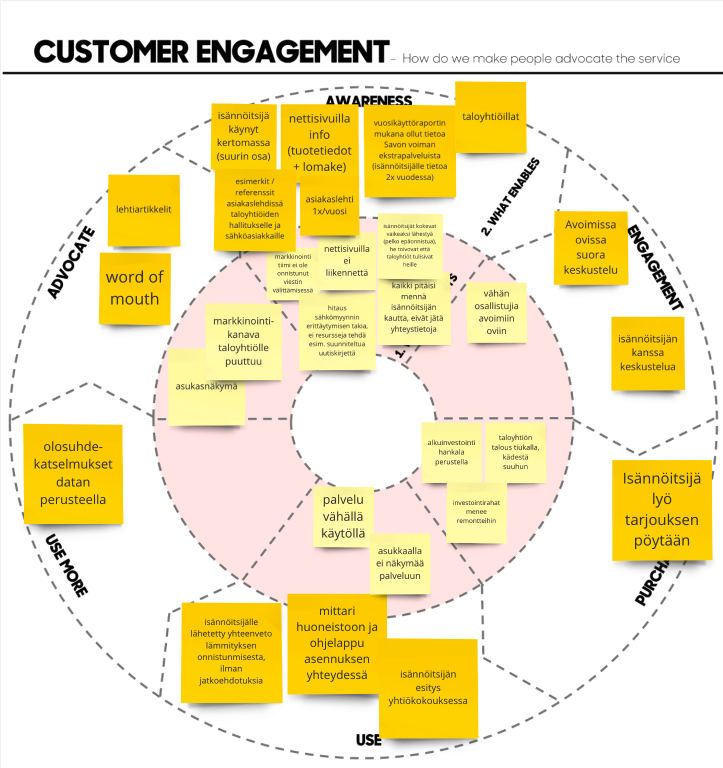
\includegraphics[width=\textwidth]{dippa/images/customer-engagement.png}
    \caption{Customer engagement canvas filled with one energy company}
    \label{fig:customer-engagement}
  \end{center}
\end{figure}

\subsubsection*{Awareness and Engagement Phases Overlap}

In the awareness phase, which is the first step, it depends on the energy company how they rise the awareness about the service. It is quite normal that the first time the housing company's chairperson hear about the service is when they receive an offer from the energy company. If that is the case, the offer usually has also some info material about the service. Another way for a housing company to know about the service is from the energy company's website where they have information about services and products that they offer. Additionally, the energy companies send newsletters and customer magazines to all of their customers where they inform their customers about new services or have some case stories featuring their services. However, it was clear that this way of doing is not that effective and it is left for the housing company board member's responsibility to then proceed with the topic.

During the awareness phase many problems were identified in addition to the previously mentioned. One issue was that the web pages do not have much of a traffic, so getting people for the right page is difficult. Moreover it was stated that marketing team should succeed to deliver the message to the customer. If the deputy landlord is responsible for discussing and also selling the service it was mentioned that they might deliver the message differently. This then leads to the situation where the energy company do not really know how the deputy landlords present the service. If the selling do not succeed the reasons behind the decision do not come into the knowledge of the energy companies. From the deputy landlords perspective, they might feel it is hard to approach the boards of the housing companies because they are afraid of failure and hope that they would approach them instead. 

Engagement is happening between the housing company board and energy companies only in rare situation. This is usually happening in open day events when the people have opportunity to discuss about the available services with the representative from the energy companies. Another form of engagement is a call after the offer is sent to discuss about the offered service more. However, it was discovered that these calls do not happen in every situations.

The main problem identified concern the fact that awareness and engagement phases are actually overlapping and there is no clear pattern or guidance on how the journey should go. Some energy companies are also lacking resources for example in marketing and then the responsibility for doing the communication is left for one person in the energy company. This leads then to the situation where closing the deals is not succeeding. Because of this it was also difficult to fill the steps after the purchase phase and the answers for them were mainly ideas how things could go if they were able to sell the service.

\section{Results from User Testing and Prototyping}

The following chapter will present the result gained from the the conducted experiments related to pricing model and personal selling. 

\subsection{Pricing Model}

In order to gain insights about pricing models and which of them is thought as the most suitable choice by the housing company's board members, the researcher and the team participated to housing company fair. There the fake ads were shown to 12 people. Eight of them were members of the board of a housing company, two were deputy landlords, one had background in housing company sales and one worked in a energy company.

Ten out of twelve people chose the pricing model that had the service fee which would be covered with the savings. Two out of twelve people did not have an opinion and three people said they would pick the investment pricing model if the housing company was wealthy otherwise the service fee with the savings.

\subsubsection*{Insights and Impact}

From this testing the biggest insight was that investment is not a good option to have as the only choice since the members of housing companies might fear to make a decision about it. However, if the housing company do have money on their account, the investment is the best option because in a long run it is more affordable.

As a result of the test, the partner company decided to move from an investment based pricing model to a pricing model which do not have investment and the service is paid with the saved costs. In addition, from this testing the case company also decided to have the service fee without investment as the main pricing model which they recommend for the partner companies.

In addition to the pricing model, the team received feedback about the advertisement and the texts in it. Related to showing the pricing, it was hoped by the test people to show price per apartment and not only for the building so it would be more understandable. Additionally, the contract period was hoped to be mentioned in the advertise. All in all the overall feedback was positive and the service was commented to be useful.

\subsection{Support for Personal Selling}

The researcher attended in a one open day event which was organised by one of the energy company partner. There the researcher was presenting the case company and working as a sales person for the energy company. The researcher approached people attending the open day with the customised offers which were done by the team for the specific housing companies.

\subsubsection*{Insights and Impact}

Attendance for an open day was not that great from the perspective of the housing companies. The researcher was able to speak only for three board members. The researcher gave the people the offer which also included the basic information about the service and let them read the paper. Afterwards, the researcher answered the questions and provided consultancy for the people if there were some unclear matters.

The researcher noticed that it was necessary to give a short presentation about the service in addition to the information which was presented in the paper. The board members were really interested in receiving the offer, because the researcher was able to give them a customized offer that stated the estimated savings in their housing company. In addition, the overall feedback about the service was positive.


 
\chapter{Discussion}
\label{chapter:discussion}

This chapter consists of the discussion about the results related to the research questions. In addition, the limitations of the study are gone through. Lastly the recommendations of future research as well actions are presented.

\section{Answers to the Research Question}

In this chapter the answers to the research question are presented and reflected to the previous literature. In addition to the answers for the research questions, the researcher suggest actions to do related to them.

\subsection{Buying Decision Making in Limited Liability Housing Company (RQ 1)}

The first research question asked about the factors which affect the buying decision making in a limited liability housing company. More specifically, the study investigated what kind of people there are in the boards of limited liability housing companies and how they operate in order to understand the motives to make decisions. In chapter 4, the factors influencing on the buying decision making were described through themes found in the interviews which were motivation of the board, role of the deputy landlord, decision making in general and board culture.

Based on the interviews, one of the biggest findings was the fact that the people who are in the board are influencing the actions and operation of the limited liability housing company the most. Issues related to the original thought that the decision making is hard found out to be more about understanding the topic being decided about rather than the decision making itself. This finding is in line with the dissertation \emph{Uncertainty in Consumer Online Search and Purchase Decision Making} made by \textcite{PurchaseDecisionMaking:2011} where it is referenced that there are two types of uncertainty in purchase decision making, knowledge uncertainty and choice uncertainty. Knowledge uncertainty means the doubts the consumers have related to their own ability to judge the service providers as well as the product itself which makes the decision making more complicated since it is then hard to do evaluate the options and it drives consumers to do more pre-purchase search. Based on the interviews it can be stated that the actual buying decision making is pretty simple once the issue being decided is made clear for everyone and there is no knowledge uncertainty.

As stated also in the chapter 2.1, the board of the limited liability housing company can make decision by themselves also without the shareholder's meeting. These decisions are usually budgeted and do not contain any big investments or they do not affect the shareholder's possessed property usage. It usually depends on the board that how and which of the decisions are presented to the shareholder's meeting. Albeit, there are situations where not that many people attend the shareholder's meeting, it is crucial to provide enough information for all in order to reach the wanted outcome.

The motivation of the board should be considered from two perspectives. First, the motivation is highly dependent on the people who are in the board and secondly, the motivation and aspirations of the board is driving the actions of the board. As mentioned previously, if the board do not have anyone who would have professional experience for example from the real estate industry, it is highly likely that the deputy landlord is then the one who is leading the limited liability housing company actions. This factor was also noticed in the thesis made by \textcite{PehkonenThesis:2012} where she researched energy efficiency related thoughts in limited liability housing companies in the area of Helsinki. Pehkonen states in the thesis that the limited liability housing companies who have professional experience or an active deputy landlord stand out from the group with activity.

The problems and needs identified in limited liability housing companies related to their operations and making buying decisions can be formed from the interviews and are as follow:
\begin{itemize}
	% You can use this command to set the items in the list closer to each other
	% (ITEM SEParation, the vertical space between the list items) 
	\setlength{\itemsep}{1pt}
	\item Deputy landlord do not always meet the needs of a housing company.
	\item Lack of workmanship inside the board leads to a situation where the goal is to keep the building as it is currently.
	\item Lack of knowledge and understanding may lead to decision making where everyone do not know what they are actually deciding.
	\item Recruiting new people to the board is hard in some cases and people do not have interest towards the housing company actions enough.
	\item Board needs professional consulting to make decision if they do not have knowledge related to the topic or they do not have the knowledge inside the board.
\end{itemize}

In conclusion the operation of the housing board is dependent of the people and their background. In addition, the housing companies are dependent on the deputy landlord for actually running the operations. The more active the board is the less important role deputy landlord usually has. What is important to notice is the fact that the decisions are made firstly in order to provide good living conditions for residents and secondly to provide them in cost effective way.

The interviews also made clear that the service provided by the case company is not applicable as it is currently for the private housing companies because the lack of knowledge and expertise. Thus, the communication about the service  as well as the product itself need to be simplified and re-though for the private housing companies since for them the concept of energy efficiency is not that well understood and it might also mean worse indoor conditions. The fear of receiving lower indoor temperatures as a result of energy efficiency was also stated by \textcite{PehkonenThesis:2012}. This observation and the interview results were the base for then creating guidance about how to sell services for limited liability housing companies as well as what needs to be considered in that scenario. These suggestions are presented in the next chapter.

\subsection{Guidance About Sales process (RQ 2)}

(discussion ristiriita että isännöitsijät toivoo aktiivisuutta taloyhtiöltä ja päinvastoin, ihmisllä ei tietoa palvelusta joten eivät myöskään osaa etsiä)

(discussion, huono kun pitää mennä tarjous / info yhdessä samassa paketissa, jolloin hirveesti infoa yhdessä lapussa).

The second research question focused on finding out what kind of sales process would help energy companies to sell services for limited liability housing companies. To answer this question the current sales process was needed to go through with customer journey mapping and then do small tests related to different phases of the journey.

Based on the research on of the most important aspect of selling services to limited liability housing company is to internalize the fact that limited liability housing company is not a business customer even though the name says limited liability company. The board of the limited liability housing company is consisting of so to say normal people who are mainly working in the board voluntarily even though they might receive a small compensation for the effort. Moreover, the energy companies should see the limited liability housing companies as actual customers and not as rate-payers, in order to understand them and to provide them services which they need.

What it comes to the presentation of the provided services there are few things which should be considered in the limited liability housing company scene. Since, one person in the board can't make decisions alone the whole presentation needs to be considered from the perspective that it also provides guidance for the one who is presenting the service for other board members. Here are listed the factors which should be in mind while designing the actual sales material. \emph{The user needs a way to:}
\begin{itemize}
\item Understand what the company is selling and why it is important.
\item Present the product for other board members
\item Make the buying decision by consulting someone professional if (s)he doesn't have the skills related to the topic
\item Know if the provided service is needed/relevant for the building
\end{itemize}

Related to the pricing of the service, it should be either service fee based or investment plus service fee. Even though, the research indicate that the service fee is more wanted among the limited liability housing company board, some companies might have more asset and are capable and willing to invest more money in the beginning to gain more benefit in the long run.

Based on the interviews and from the testing, it came clear that the deputy landlord is the trusted person among the board of limited liability housing companies. Moreover, one deputy landlord handles usually many limited liability housing companies at once, meaning that they reach many potential customers and have relationship with them already. Thus, deputy landlord could be a potential way to sell new services for limited liability housing company if they believe and see value in the service themselves. This however is not as easy as it sounds because there was found to be a conflict where some deputy landlords wish limited liability housing companies to be active and vice versa. In this situation it is then hard to identify, who should be the one to make the limited liability housing company operation better.

In the context of selling a service which is totally new in the market the boards who are trendsetters, as presented in the chapter 4, should be identified. Since, they are the most proactive it could be also the easiest way to sell them the service first. Through this then, the care takers and responsible would follow the trendsetters. One of the issues in selling something new is that people do not have knowledge about it, so it is hard to start even looking for it. In this situation, the responsibility to provide such information lies on the service provider. Also according to \textcite{PurchaseDecisionMaking:2011} expert consumers do not need information and they do not search it which is also typical for novice users. However, the reason why novice consumers do not search information is because they lack the ability to do so. Additionally, the consumers who are in the middle are easiest to target since they can be influenced via advertises with the least effort. ( tähän viittaus kirjallisuuteen trend settereistä tai early adoptereista the part of early adapters are a ) 

The analyze of the interviews brought up also the fact that energy efficiency and green values are not seen as important or understood the way professionals do. In addition, the interviewees listed that their responsibility is to provide good living conditions to all residents. Having these facts in mind the current value proposition could be transformed from saving energy in a energy efficient way of heating towards providing stable and equal living conditions to all residents in the apartment building.

\section{Limitations of the study}

The study has limitations which should be acknowledged. Related to the data collection process, the researched did the interviews alone and it is possible that even though the interview questions were open ended the interviewer directed the answers of the interviewee. The generalizability of the interview results is geographically uncertain since the interviewees all lived in the capital area of Finland, still the interviewees represented well different age groups, different levels of experience in the board as well as gender.

In addition, it is possible that the interviewees' answers were affected by the desire to please the interviewer. Nevertheless, the interviewees talked openly about their feelings and motivations related to working in the limited liability housing board even though in some cases they were negative and critical, which indicate that the answers represent their opinions in real life. 

During the data analyze phase only one researcher analyzed the interviews and because of that the previous knowledge and perspectives could have affected how the researcher analyzed and categorized the interviews. To be noted, the researched did not have any experience on being part of the limited liability housing board so she did not have any strong opinions or own experiences that could have highly affected the analysis.

Because of the time span of the thesis, the researcher did not have enough time to iterate the tests according to the design science research, so the suggestions would need more testing to be generalized in larger context. In addition, it is hard to measure if the research results helped to reduce customer acquisition costs, reduce lead times and increase sales since the test were concentrating on small parts of the whole customer journey compared to contemplating it as a whole.

\section{Future work}

The future work and research could be about researching more about issues and needs that the limited liability housing companies has related to heating and energy efficiency. Since, there are already few heating optimization services in the market it could be beneficial to do user research with the ones who are already using the service. Through the researc, the company would get more information on what is really important for the limited liability housing company and what brings them value and benefits.

In addition, the future work should concentrate on finding out how the deputy landlords would use the service and how the whole maintenance chain could be designed around the service in order to be fully predicting.
(discuss tuleva tutkimus oikeasta tuotteesta taloyhtiöille)
mitä ongelmia lämmityksessä
tarkemmin energiatehokkuuteen liittyvää juttuu



% Load the bibliographic references
% ------------------------------------------------------------------
% You can use several .bib files:
% \bibliography{thesis_sources,ietf_sources}
% \bibliography{sources}
\printbibliography

% Appendices go here
% ------------------------------------------------------------------
% If you do not have appendices, comment out the following lines
\appendix
\chapter{First appendix}
\label{chapter:first-appendix}

This is the first appendix. You could put some test images or verbose data in an
appendix, if there is too much data to fit in the actual text nicely.

For now, the Aalto logo variants are shown in Figure~\ref{fig:aaltologo}.



% End of document!
% ------------------------------------------------------------------
% The LastPage package automatically places a label on the last page.
% That works better than placing a label here manually, because the
% label might not go to the actual last page, if LaTeX needs to place
% floats (that is, figures, tables, and such) to the end of the 
% document.
\end{document}
